% (c)~2014 Dimitrios Vrettos - d.vrettos@gmail.com
% (c)~2014 Claudio Carboncini - claudio.carboncini@gmail.com
% (c)~2015 Daniele Zambelli daniele.zambelli@gmail.com
% (c)~2015 Maria Antonietta Pollini

% (c) 2014 Daniele Zambelli - daniele.zambelli@gmail.com

\newcommand{\quadratopitagorico}[3]{%
  \coordinate (a) at (0, 0);
  \coordinate (b) at (#1, 0);
  \coordinate (c) at (#1, #1);
  \coordinate (d) at (0, #1);
% \colorlet{anglecolor}{green!50!black}

  \begin{scope}[line join=round, line cap=round]
    \draw[thick, Maroon!50!black] (a)--(b)
          node [black, sloped, midway, below] {#2} -- (c) -- cycle 
          node [black, sloped, midway, above] {#3};
    \draw[thick, Maroon!50] (a)--(d)--(c);
%     \draw [->, anglecolor, thick](#1*.3, 0) arc(0:45:#1*.3);
    \draw [->, thick](#1*.3, 0) arc(0:45:#1*.3);
%     \draw (#1*.45, #1*.15) node [anglecolor] {$45 \text{°}$};
    \draw (#1*.45, #1*.15) node {$45 \text{°}$};
  \end{scope}
}


\newcommand{\triequipitagorico}[1]{%
  \coordinate (a) at (0, 0);
  \coordinate (m) at (#1/2, 0);
  \coordinate (b) at (#1, 0);
  \coordinate (c) at (#1/2, #1 * 0.8660254);

  \begin{scope}[line join=round, line cap=round]
    \draw[thick, Maroon!50!black] (a)--
          (m)
          node [black, sloped, midway, below] {$\frac{l}{2}$} -- 
          (c)
          node [black, sloped, midway, above, xshift=-10pt] 
               {$l \cdot \frac{\sqrt{3}}{2}$} -- 
          cycle 
          node [black, midway, above left] {$l$};
    \draw[thick, Maroon!50] (m)--(b)--(c);
%     \draw [->, anglecolor, thick](#1*.3, 0) arc(0:60:#1*.3);
    \draw [->, thick](#1*.15, 0) arc(0:60:#1*.15);
%     \draw (#1*.45, #1*.15) node [anglecolor] {$60 \text{°}$};
    \draw (#1*.25, #1*.08) node  {$60 \text{°}$};
  \end{scope}
}


% \begin{figure}[h]
% \begin{minipage}{.40\textwidth}
% 
% \end{minipage}
% \begin{minipage}{.60\textwidth}
% \begin{inaccessibleblock}[?]
% \centering
%   \input{\folder lbr/?.pgf}
%   \caption{?.} \label{fig:?_?}
% \end{inaccessibleblock}
% \end{minipage}
% \end{figure}

% \begin{wrapfloat}{figure}{r}{0pt}
% \includegraphics[scale=0.35]{img/?.png}
% \caption{?}
% \label{fig:?_?}
% \end{wrapfloat}
% 
% \begin{center} \input{\folder lbr/?.pgf} \end{center}

\begin{comment}

\begin{inaccessibleblock}[]
\begin{center}
  \
\end{center}
\end{inaccessibleblock}
\end{comment}

\begin{comment}
 
 \begin{minipage}{.45\textwidth}
  
 \end{minipage}
 \begin{minipage}{.25\textwidth}
  
 \end{minipage}
 \begin{minipage}{.3\textwidth}
  
 \end{minipage}
 
\end{comment}

\chapter{Disequazioni}

\section{Risoluzione delle disequazioni di secondo grado}
\label{sec:diseq_secondo_grado}

Una disequazione di secondo grado si presenta in una delle seguenti forme:
\[ax^2+bx+c<0;\quad ax^2+bx+c\le 0;\quad ax^2+bx+c\ge0;\quad ax^2+bx+c> 0\]

Ricordiamo che risolvere una disequazione in un'incognita significa 
determinare l'insieme dei valori da attribuire all'incognita affinché la 
disequazione sia verificata.
Come per le disequazioni di primo grado anche per quelle di secondo grado
dobbiamo studiare il segno del trinomio e poi individuare l'insieme soluzione.

\subsection{Studio del segno di un trinomio di secondo grado}
\label{subsec:diseq_trinomio}

Per studiare il segno di un polinomio di secondo grado seguiamo un 
procedimento in due passi:

\begin{enumerate}
 \item Equazione associata
Risolvendo l'equazione associata al polinomio troviamo gli zeri della 
funzione cioè i punti in cui il grafico della funzione incontra l'asse~x. 

A seconda del valore del discriminante l'equazione può avere 
nessuna soluzione reale (\(\Delta<0\)), 
soluzioni reali coincidenti (\(\Delta=0\)), 
soluzioni reali distinte (\(\Delta>0\)).

 \item Grafico della funzione associata
Disegnando il grafico della funzione associata al polinomio si individuano 
gli intervalli in cui il polinomio è positivo, il grafico è sopra l'asse~x 
o negativo, il grafico è sotto l'asse~x.

Se il coefficiente del termine di secondo grado è minore di zero (\(a<0\)) 
la parabola ha la concavità rivolta verso il basso, se è maggiore di zero 
(\(a>0\)) la parabola ha la concavità rivolta verso l'alto. 
\end{enumerate}

% \begin{exrig}
\begin{esempio}
Studiare i segno del polinomio: \(x^2-2x-3\)

\begin{enumerate}
 \item
  Equazione Associata:~\(x^2-2x-3=0 \sRarrow 
                        \left(x-3 \right)\left(x+1\right)=0 \sRarrow 
                        x_1=-1~\cup~x_2=+3\)
 \item 
  \begin{minipage}{.45\textwidth}
  Funzione Associata: \(y = x^2-2x-3 \quad \rightarrow\)
  \end{minipage}
  \begin{minipage}{.30\textwidth}
  \parabolaamadma{-1}{3}
  \end{minipage}
\end{enumerate}

\end{esempio}

Una volta studiato il segno del polinomio, risolvere una disequazione nella 
forma \(f(x) \lessgtr 0\) consiste nell'aggiungere un ulteriore passo 
piuttosto banale: individuare l'insieme soluzione.

\begin{esempio}
Risolvi le seguente disequazioni utilizzando lo studio del segno del trinomio 
di secondo grado.

\begin{itemize}
\item \(x^2+x-2>0$.

\begin{enumerate}
 \item
  Equazione Associata:~\(x^2+x-2=0 \sRarrow 
                        \left(x-1 \right)\left(x+2\right)=0 \sRarrow 
                        x_1=-2~\cup~x_2=+1\)
 \item 
  \begin{minipage}{.45\textwidth}
  Funzione Associata: \(y = x^2+x-2 \quad \rightarrow\)
  \end{minipage}
  \begin{minipage}{.30\textwidth}
  \parabolaamadma{-2}{+1}
  \end{minipage}
 \item 
 Insieme soluzione\\
 
  \begin{minipage}{.32\textwidth}
  Forma grafica\\[-.7em]
  
 \begin{center}
   \inteaa{4}{-1.5}{+1.5}{-2}{+1}
  \vspace{.4em}
 \end{center}
  \end{minipage}
  \begin{minipage}{.32\textwidth}
  Espressione con i predicati\\[-.3em]
  
 \begin{center}
  \(x<-2 \sor x>+1\)
  \vspace{1em}
 \end{center}
  \end{minipage}
  \begin{minipage}{.32\textwidth}
  Espressione con le parentesi\\[-.3em]
  
 \begin{center}
  \(\intervaa{-\infty}{-2}~\cup~\intervaa{1}{-\infty}\)
  \vspace{.8em}
 \end{center}
  \end{minipage}
\end{enumerate}

\item \(x^2-4x+4\le0$.

\begin{enumerate}
 \item
  Equazione Associata:~\(x^2-4x+4=0 \sRarrow 
                        \left(x-2 \right)^2=0 \sRarrow 
                        x_{1,2}=+2\)
 \item 
  \begin{minipage}{.45\textwidth}
  Funzione Associata: \(y = x^2-4x+4 \quad \rightarrow\)
  \end{minipage}
  \begin{minipage}{.30\textwidth}
  \parabolaamadz{+2}
  \end{minipage}
 \item 
 Insieme soluzione\\
 
  \begin{minipage}{.32\textwidth}
  Forma grafica\\[-.7em]
  
 \begin{center}
  \puntoc{4}{0}{+2}
  \vspace{.4em}
 \end{center}
  \end{minipage}
  \begin{minipage}{.32\textwidth}
  Espressione con i predicati\\[-.3em]
  
 \begin{center}
  \(x=2\)
  \vspace{1em}
 \end{center}
  \end{minipage}
  \begin{minipage}{.32\textwidth}
  Espressione con le parentesi\\[-.3em]
  
 \begin{center}
  \(\lbrace +2 \rbrace\)
  \vspace{.8em}
 \end{center}
  \end{minipage}
\end{enumerate}

\item \(-x^2+2x-7>0$.

\begin{enumerate}
 \item
  Equazione Associata:~\(-x^2+2x-7=0 \sRarrow 
                        \dfrac{\Delta}{4} = -6 \sRarrow 
                        \text{N.H.S.R.}\)
 \item 
  \begin{minipage}{.45\textwidth}
  Funzione Associata: \(y = -x^2+2x-7 \quad \rightarrow\)
  \end{minipage}
  \begin{minipage}{.30\textwidth}
  \parabolaamidmi
  \end{minipage}
 \item 
 Insieme soluzione\\
 
  \begin{minipage}{.32\textwidth}
  Forma grafica\\[-.7em]
  
 \begin{center}
  \intv{8}
  \vspace{.4em}
 \end{center}
  \end{minipage}
  \begin{minipage}{.32\textwidth}
  Espressione con i predicati\\[-.3em]
  
 \begin{center}
  \(\nexists x \in \R\)
  \vspace{1em}
 \end{center}
  \end{minipage}
  \begin{minipage}{.32\textwidth}
  Espressione con le parentesi\\[-.3em]
  
 \begin{center}
  \(\emptyset\)
  \vspace{.8em}
 \end{center}
  \end{minipage}
\end{enumerate}

\item \(2x^2-5 \le 0\).

\begin{enumerate}
 \item
  Equazione Associata:~\(2x^2-5=0 \sRarrow 
                        x_{1, 2}= \mp \sqrt{\dfrac{5}{2}}\)
 \item 
  \begin{minipage}{.45\textwidth}
  Funzione Associata: \(y = 2x^2-5 \quad \rightarrow\)
  \end{minipage}
  \begin{minipage}{.30\textwidth}
  \parabolaamadma{-\sqrt{\dfrac{5}{2}}}{+\sqrt{\dfrac{5}{2}}}
  \end{minipage}
 \item 
 Insieme soluzione\\
 
  \begin{minipage}{.32\textwidth}
  Forma grafica\\[-.7em]
  
 \begin{center}
  \inticc{4}{-1.5}{+1.5}{-\sqrt{\dfrac{5}{2}}}{+\sqrt{\dfrac{5}{2}}}
  \vspace{.4em}
 \end{center}
  \end{minipage}
  \begin{minipage}{.32\textwidth}
  Espressione con i predicati\\[-.3em]
  
 \begin{center}
  \(-\sqrt{\dfrac{5}{2}} \le x \le +\sqrt{\dfrac{5}{2}}\)
  \vspace{1em}
 \end{center}
  \end{minipage}
  \begin{minipage}{.32\textwidth}
  Espressione con le parentesi\\[-.3em]
  
 \begin{center}
  \(\intervcc{-\sqrt{\dfrac{5}{2}}}{+\sqrt{\dfrac{5}{2}}}\)
  \vspace{.8em}
 \end{center}
  \end{minipage}
\end{enumerate}

\item \(-3x^2 + 2x > 0\).

\begin{enumerate}
 \item
  Equazione Associata:~\(-3x^2 + 2x=0 \sRarrow 
                        x_{1}= 0 \sand x_{2}= \dfrac{2}{3}\)
 \item 
  \begin{minipage}{.45\textwidth}
  Funzione Associata: \(y = -3x^2 + 2x \quad \rightarrow\)
  \end{minipage}
  \begin{minipage}{.30\textwidth}
  \parabolaamidma{0}{+\dfrac{2}{3}}
  \end{minipage}
 \item 
 Insieme soluzione\\
 
  \begin{minipage}{.32\textwidth}
  Forma grafica\\[-.7em]
  
 \begin{center}
  \intiaa{4}{-1.5}{+1.5}{0}{+\dfrac{2}{3}}
  \vspace{.4em}
 \end{center}
  \end{minipage}
  \begin{minipage}{.32\textwidth}
  Espressione con i predicati\\[-.3em]
  
 \begin{center}
  \(0 < x < +\dfrac{2}{3}\)
  \vspace{1em}
 \end{center}
  \end{minipage}
  \begin{minipage}{.32\textwidth}
  Espressione con le parentesi\\[-.3em]
  
 \begin{center}
  \(\intervaa{0}{+\dfrac{2}{3}}\)
  \vspace{.8em}
 \end{center}
  \end{minipage}
\end{enumerate}

\end{itemize}
\end{esempio}

% %%%%%%%%%%%%%%%%%%%%%%%%%%%%%%
% \section{Segno del trinomio a coefficienti letterali}
% Consideriamo il trinomio \(t=kx^2+3x-7\) di secondo grado avente il primo 
% coefficiente dipendente dal parametro \(k$. Come possiamo stabilire il 
% segno 
% di 
% questo trinomio, al variare di \(k$?
% Sappiamo che stabilire il segno di un trinomio significa determinare i 
% valori 
% reali che attribuiti alla variabile indipendente \(x\) rendono il trinomio 
% positivo, nullo o negativo. Evidentemente per valori reali diversi di \(k\) 
% avremo 
% una diversa disequazione da risolvere; dobbiamo dunque cercare di 
% analizzare 
% come varia il trinomio a seconda dei valori di \(k\) e in seguito studiare 
% il 
% segno del trinomio ottenuto. Questa analisi di situazioni diverse è la 
% \textit{discussione del trinomio a coefficienti parametrici}.
% 
% %%%%%%%%%%%%%%%%%%%%%%%%%%%%%%
% \conclusione Una disequazione di secondo grado si presenta sempre in una 
% delle 
% seguenti forme: \({ax}^2+{bx}+c>0\), \({ax}^2+{bx}+c\ge 0\), 
% \({ax}^2+{bx}+c<0\), 
% \({ax}^2+{bx}+c\le 0\) possiamo sempre supporre positivo il primo 
% coefficiente 
% e, 
% anche se incompleta, per l'equazione associata possiamo sempre pensare ai 
% tre 
% casi generati dal segno del discriminante \(\Delta =b^2-4{ac}$. Pertanto 
% avremo:
% 
% %%%%%%%%%%%%%%%%%%%%%%%%%%%%%
% % \begin{exrig}
% \begin{esempio}
% Stabilire il segno di \(t=kx^2+3x-7\) al variare di \) k \(.
% 
% Prendiamo in considerazione il segno del primo coefficiente e il segno del 
% discriminante dell'equazione associata \(kx^2+3x-7=0$. Il primo 
% coefficiente è 
% maggiore di zero per \(k>0$. Il discriminante \(\Delta =9+28k\) è maggiore 
% di 
% zero 
% per \(k>-\frac 9{28}$. Rappresentiamo la loro reciproca situazione:
% \begin{center}
% %%%%%%%%%%%%%%%%%%%%%%%%%%%%%%
% \begin{threeparttable}
% \begin{tabular}{lllll}
% \toprule
% Delta & \(ax^2+bx+c>0$& \(ax^2+bx+c\ge0$& \(ax^2+bx+c<0\) & 
% \(ax^2+bx+c\le0$\\
% \midrule
%  \(\Delta >0^{*}$& \) x<x_1\vee x>x_2 \) & \) x\le x_1\vee x\ge x_2 \(& \) 
% x_1<x<x_2 
% \(&\) x_1\le x\le x_2 \(\\
% \(\Delta =0^{**}$& \(\forall x\in \insR-\{x_1\} \) & \) \forall x\in \insR 
% \(& \) 
% \IS=\emptyset \(&\) x=x_1=x_2 \(\\
% \(\Delta <0^{***}$&\) \forall x\in \insR \) & \) \forall x\in \insR \(& \) 
% \IS=\emptyset \(&\) \IS=\emptyset \(\\
% \bottomrule
% \end{tabular}
% \begin{tablenotes}
% \item [*] L'equazione associata ha 2 soluzioni reali distinte: \(x=x_1\vee 
% x=x_2$.
% \item [**] L'equazione associata ha 2 soluzioni reali coincidenti: 
% \(x=x_1=x_2$.
% \item [***] L'equazione associata non ha soluzioni reali.
% \end{tablenotes}
% \end{threeparttable}
% \end{center}
% %%%%%%%%%%%%%%%%%%%%%%%%%%%%%%
%  % (c) 2013 Claudio Carboncini - claudio.carboncini@gmail.com
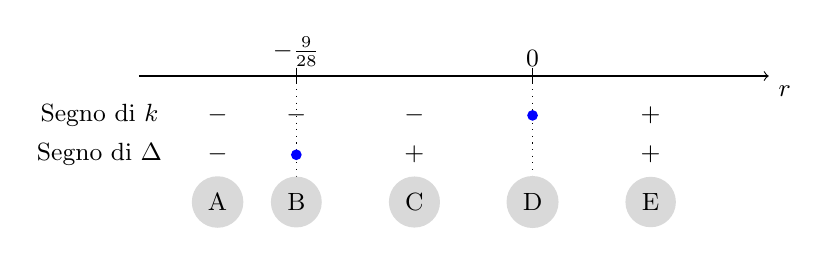
\begin{tikzpicture}[font=\small,x=10mm, y=10mm]

\draw[->] (0,0) -- (8,0) node [below right] () {$r$};

\foreach \x in {2,5}{
\draw(\x,3pt)--(\x,-3pt);
\begin{scope}[dotted]
\draw (\x,0) -- (\x,-1.5);
\end{scope}}
\node[] at (-.5,-0.5) {Segno di $k$};
\node[] at (-.5,-1) {Segno di $\Delta$};
\node[above]  at (2,0) {$-\frac{9}{28}$};
\node[above]  at (5,0) {$0$};
\node[] at (1,-0.5) {$-$};
\node[] at (2,-0.5) {$-$};
\node[] at (3.5,-0.5) {$-$};
\node[] at (6.5,-0.5) {$+$};
\node[] at (1,-1) {$-$};
\node[] at (3.5,-1) {$+$};
\node[] at (6.5,-1) {$+$};
\node [circle,fill=gray!30](A) at (1,-1.6) {A};
\node [circle,fill=gray!30](B) at (2,-1.6) {B};
\node [circle,fill=gray!30](C) at (3.5,-1.6) {C};
\node [circle,fill=gray!30](D) at (5,-1.6) {D};
\node [circle,fill=gray!30](E) at (6.5,-1.6) {E};

\begin{scope}[blue,thick]
\draw[fill=blue] (5,-.5)circle (1.5pt);
\draw[fill=blue] (2,-1)circle (1.5pt);
\end{scope}

\end{tikzpicture}

% % \end{center}
% \vspazio\ovalbox{\risolvii \ref{ese:4.1}, \ref{ese:4.2}, \ref{ese:4.3}, 
% \ref{ese:4.4}, \ref{ese:4.5}, \ref{ese:4.6}}
% 
% \end{esempio}
% 
% %%%%%%%%%%%%%%%%%%%%%%%%%%%%%%
% % \end{exrig}

\section{Disequazioni polinomiali di grado superiore}
\label{sec:diseq_grado_superiore}

\begin{procedura}
Risolvere le disequazioni di grado superiore:
\begin{enumeratea}
\item scomponi il polinomio di grado \(n\) in fattori di primo e secondo 
grado;
\item studia il segno dei singoli fattori;
\item costruisci la tabella dei segni;
\item applica la regola dei segni per calcolare il segno della frazione;
\item cerca gli intervalli in cui il polinomio dato assume il segno richiesto.
\item rappresenta, con i diversi metodi visti, gli intervalli che 
 risolvono la disequazione.
\end{enumeratea}
\end{procedura}

Applichiamo la procedura ai seguenti esempi.

% \begin{exrig}
\begin{esempio}
 \[p(x)=-2x^3+3x^2+8x-12 \le 0\]

In questo caso dobbiamo risolvere una disequazione di terzo grado. 
Possiamo ridurre la difficoltà scomponendo in fattori il polinomio in modo da 
ottenere il prodotto di più polinomi di primo grado: 

\begin{align*}
P(x) = -2x^3+3x^2+8x-12 &= x^2(-2x+3)-4(-2x+3) = \\
                        &= (x^2-4)(-2x+3)
\end{align*}

A questo punto possiamo studiare il segno dei fattori e, applicando la regola 
dei segni di un prodotto, trovare il segno del polinomio iniziale e risolvere 
la disequazione.

Studiamo il segno di ogni singolo fattore:
\begin{itemize}

 \item segno di \(x^2-4\)\\
 \begin{minipage}{.35\textwidth}
  E.A.:~\(x^2-4=0 \sRarrow x=\mp 2\)
 \end{minipage}
 \begin{minipage}{.25\textwidth}
  F.A.:~\(y=x^2-4 \sRarrow\)
 \end{minipage}
 \begin{minipage}{.38\textwidth}
  \begin{inaccessibleblock}[parabola concavità verso l'alto, interseca 
l'asse~x in -2 e +2]
  \parabolaamadma{-2}{+2}
\end{inaccessibleblock}
 \end{minipage}
 
 \item  segno di \(-2x+3\)\\
 \begin{minipage}{.35\textwidth}
  E.A.:~\(-2x+3=0 \sRarrow x=\dfrac{3}{2}\)
  \vspace{1.8em}
 \end{minipage}
 \begin{minipage}{.25\textwidth}
  F.A.:~\(y=-2x+3 \sRarrow \)
  \vspace{1.8em}
 \end{minipage}
 \begin{minipage}{.38\textwidth}
  \begin{inaccessibleblock}[retta decrescente con zero in~3/2]
%   \vspace*{1.7em}
  \rettammi{5}{\dfrac{3}{2}}
\end{inaccessibleblock}
 \end{minipage}
 
 \item Con la regola dei segni calcolo il segno del prodotto:

\begin{inaccessibleblock}[Grafo con i segni]
  \begin{center}
  \segnoprodottoa
  \end{center}
\end{inaccessibleblock}

 \item Quindi i valori di~\(x\) che rendono vera la disequazione, cioè i 
valori
  che rendono~\(f(x)\) non positivo, sono quelli 
  che si trovano a sinistra di~\(-2\) oppure che si trovano a destra 
di~\(+3$.\\

  \begin{minipage}{.32\textwidth}
  Forma grafica\\[-1.2em]
  
\begin{inaccessibleblock}[Grafo con i segni]
  \begin{center}
  \solprodottoa
  \end{center}
\end{inaccessibleblock}
\vspace{.1em}

  \end{minipage}
  \begin{minipage}{.32\textwidth}
  Espressione con i predicati\\[-.3em]
  
 \begin{center}
  \(-2 \le x \le +\dfrac{3}{2} \sor x \ge +2\)
  \vspace{1em}
 \end{center}
  \end{minipage}
  \begin{minipage}{.32\textwidth}
  Espressione con le parentesi\\[-.3em]
  
 \begin{center}
  \(\intervcc{-2}{+\dfrac{3}{2}}~\cup~\intervca{+2}{+\infty}\)
  \vspace{.8em}
 \end{center}
  \end{minipage}
  
\end{itemize}

\end{esempio}

\begin{esempio}
Data la disequazione 
\[-2x(3-2x)-3x^2\left(2-\dfrac{3}{2}x\right) \ge 
  5\left(2x^2-\dfrac{3}{10}x\right)\] 
determina il suo \(\IS\)

Osserviamo che la disequazione proposta è polinomiale di terzo grado; 
esegui i calcoli per portarla alla forma \(p(x)\ge 0$: 
\vspace{3em}

Scomponendo in fattori si ottiene: \(x\cdot (3x^2-8x-3)\ge 0\). 

A questo punto possiamo studiare il segno dei fattori e, applicando la regola 
dei segni di un prodotto, trovare il segno del polinomio iniziale e risolvere 
la disequazione.

Studiamo il segno di ogni singolo fattore:
\begin{itemize}

 \item segno di \(3x^2-8x-3\)\\
 \begin{minipage}{.35\textwidth}
  E.A.:~\(3x^2-8x-3=0\)
  
  \(x_1=\dots \quad x_2=\dots\)
 \end{minipage}
 \begin{minipage}{.25\textwidth}
  F.A.:~\(y=3x^2-8x-3\)
 \end{minipage}
 \begin{minipage}{.38\textwidth}
  \begin{inaccessibleblock}[parabola concavità verso l'alto, interseca 
l'asse~x in -2 e +2]
  \parabolaamadma{}{}
\end{inaccessibleblock}
 \end{minipage}
 
 \item  segno di \(x\)\\
 \begin{minipage}{.35\textwidth}
  E.A.:~\(x=0\)
  \vspace{1.8em}
 \end{minipage}
 \begin{minipage}{.25\textwidth}
  F.A.:~\(y=x\)
  \vspace{1.8em}
 \end{minipage}
 \begin{minipage}{.38\textwidth}
  \begin{inaccessibleblock}[retta decrescente con zero in~3/2]
%   \vspace*{1.7em}
  \rettamma{5}{}
\end{inaccessibleblock}
 \end{minipage}
 
 \item Con la regola dei segni calcolo il segno del prodotto:

\begin{inaccessibleblock}[Grafo con i segni]
  \begin{center}
  \segnoprodottob
  \end{center}
\end{inaccessibleblock}

 \item Quindi i'\(\IS\) è:\\

  \begin{minipage}{.32\textwidth}
  Forma grafica\\[-1.2em]
  
\begin{inaccessibleblock}[Grafo con i segni]
  \begin{center}
  \disegno{\assex{-4}{+4}{0}}
  \end{center}
\end{inaccessibleblock}
\vspace{.1em}

  \end{minipage}
  \begin{minipage}{.32\textwidth}
  Espressione con i predicati\\[2.5em]
  
  \end{minipage}
  \begin{minipage}{.32\textwidth}
  Espressione con le parentesi\\[2.5em]
  
  \end{minipage}
  
\end{itemize}

\end{esempio}

\begin{esempio}
Un numero è tale che aggiungendo al suo cubo il suo quadruplo si ottiene 
un numero maggiore del triplo del suo quadrato aumentato di~\(12$. Determina 
l'insieme soluzione del problema.

La richiesta del problema implica la ricerca dell'Insieme Soluzione della 
disequazione \(x^3+4x>3x^2+12\), di terzo grado nella variabile~\(x$. 
Scriviamo la disequazione in forma canonica, applicando i principi di 
equivalenza: 
\[x^3-3x^2+4x-12>0\]. 
Si tratta di una disequazione polinomiale di terzo grado.

Procediamo nella scomposizione in fattori del polinomio:
\[p(x)=x^3-3x^2+4x-12 = x^2 \left(x-3\right)+4 \left(x-3\right) =
      \left(x^2+4\right) \left(x-3\right)\]
Ora possiamo determinare il segno dei vari fattori, ma se siamo 
sufficientemente acuti e pigri possiamo osservare che il primo fattore sarà 
sempre positivo (perché?) quindi il segno del polinomio è equivalente al 
segno del secondo fattore che si determina molto rapidamente \dots.
\end{esempio}

\begin{esempio}
Risolvi la disequazione: \(1-81x^4<0\)

Il binomio a primo membro può essere scomposto in fattori irriducibili in due 
passi:
\[1-81x^4 = \left(1-9x^2\right)\left(1+9x^2\right)=
  \left(-9x^2+1\right)\left(9x^2+1\right)\]
Anche qui possiamo usare un po' di furbizia e calcolare la soluzione molto 
rapidamente.
\end{esempio}

\begin{esempio}
Risolvere la disequazione: \(x^4-4x^2-45 \ge 0\)

Il trinomio al primo membro è di quarto grado ma sappiamo che con la 
sostituzione: 
\(x^2=z\)

può essere ricondotto al trinomio di secondo grado:
\(z^2-4z-45 \ge 0\)

la cui scomposizione in fattori risulta:
\(\left(z-9\right)\left(z+5\right)\)

quindi la disequazione assegnata diventa: 
\((x^2-9)(x^2+5) \ge 0\)

Completa la soluzione della disequazione.
\end{esempio}

% \end{exrig}
% \vspazio\ovalbox{\risolvii \ref{ese:4.32}, \ref{ese:4.33}, \ref{ese:4.34}, 
% \ref{ese:4.35}, \ref{ese:4.36}, \ref{ese:4.37}, \ref{ese:4.38}, 
% \ref{ese:4.39}, 
% \ref{ese:4.40}, \ref{ese:4.41}, \ref{ese:4.42}, \ref{ese:4.43}, \ref 
% {ese:4.44},}
% 
% \vspazio\ovalbox{\ref{ese:4.45}, \ref{ese:4.46}, \ref{ese:4.47}, 
% \ref{ese:4.48}, 
% \ref{ese:4.49}, \ref{ese:4.50}, \ref{ese:4.51}, \ref{ese:4.52}, 
% \ref{ese:4.53}, 
% \ref{ese:4.54}, \ref{ese:4.55}, \ref{ese:4.56}, \ref{ese:4.57}}

% \newpage %----------------------------------------------

\section{Disequazioni fratte}
\label{sec:diseq_fratte}

Ricordiamo che una disequazione è \emph{frazionaria} o \emph{fratta} quando 
il suo denominatore contiene l'incognita. 

\begin{osservazione}
 \begin{itemize*}
\item studiare il segno di una espressione letterale significa stabilire in 
quale insieme si trovano i valori della variabile che rendono 
l'espressione negativa, nulla o positiva;
\item ogni espressione contenente operazioni tra frazioni algebriche ha in 
generale come risultato una frazione algebrica;
\item nello studiare il segno terremo conto anche del campo di esistenza 
della funzione.
\end{itemize*}
\end{osservazione}

Per risolvere una disequazione fratta si può applicare la seguente procedura 
quasi identica a quella che si utilizza per le funzioni scomponibili in 
fattori.

\begin{procedura}
Soluzione di una disequazione frazionaria:
\begin{enumeratea}
\item trasporta tutti i termini al primo membro e scrivilo sotto forma di 
 un'unica frazione:\\
\[\frac{N(x)}{D(x)} \lessgtr 0\]
\item scomponi in fattori numeratore e denominatore;
\item studia il segno di ogni fattore;
\item costruisci la tabella dei segni, 
\emph{ricordandosi di indicare con una crocetta gli zeri del denominatore};
\item applica la regola dei segni per calcolare il segno della frazione;
\item individua gli intervalli in cui la frazione assume il segno richiesto;
\item rappresenta, con i diversi metodi visti, gli intervalli che 
 risolvono la disequazione.
\end{enumeratea}
\end{procedura}

Vediamo attraverso alcuni esempi come procedere.

\begin{esempio}
 \[\frac{2}{x-7} \ge \frac{3}{x+4}\]

Per prima cosa dobbiamo scrivere la disequazione in forma normale:
 \[\frac{2}{x-7} - \frac{3}{x+4} \ge 0 \Rightarrow 
   \frac{2(x+4) - 3(x-7)}{(x-7)(x+4)} = 
   \frac{2 x +8 -3x +21}{(x-7)(x+4)} =
   \frac{-x +29}{x^2-3x-28} \ge 0\]

A questo punto possiamo studiare il segno dei fattori e, applicando la regola 
dei segni di un prodotto, trovare il segno della disequazione fratta.

\begin{itemize}
 \item Studiamo il segno di ogni singolo fattore:

\begin{itemize}

 \item  segno di \(-x +29\)\\
 \begin{minipage}{.35\textwidth}
  E.A.:~\(-x +29=0 \sRarrow x=29\)
  \vspace{1.8em}
 \end{minipage}
 \begin{minipage}{.25\textwidth}
  F.A.:~\(y=-x +29 \sRarrow \)
  \vspace{1.8em}
 \end{minipage}
 \begin{minipage}{.38\textwidth}
  \begin{inaccessibleblock}[retta decrescente con zero in~3/2]
%   \vspace*{1.7em}
  \rettammi{5}{29}
\end{inaccessibleblock}
 \end{minipage}
 
 \item segno di \(x^2-3x-28\)\\
 \begin{minipage}{.35\textwidth}
  E.A.:~\(x^2-3x-28=0 \sRarrow \) \\
  \(x_1=-4 \sor x_2=7\)
 \end{minipage}
 \begin{minipage}{.25\textwidth}
  F.A.:\\
  \(y=x^2-3x-28 \sRarrow\)
 \end{minipage}
 \begin{minipage}{.38\textwidth}
  \begin{inaccessibleblock}[parabola concavità verso l'alto, interseca 
l'asse~x in -4 e +7]
  \parabolaamadma{-4}{+7}
\end{inaccessibleblock}
 \end{minipage}
 
\end{itemize}
 \item Con la regola dei segni calcoliamo il segno del prodotto:

\begin{inaccessibleblock}[Grafo con i segni]
  \begin{center}
  \segnofrazionea
  \end{center}
\end{inaccessibleblock}

 \item Quindi i valori di~\(x\) che rendono vera la disequazione, cioè i 
valori
  che rendono~\(f(x)\) non negativo, sono quelli 
  che si trovano a sinistra di~\(-4\) oppure che sono compresi 
  tra~\(+7$.\\

  \begin{minipage}{.32\textwidth}
  \vspace{.7em}
  Forma grafica\\ [-.8em]
  
\begin{inaccessibleblock}[Grafo con i segni]
  \begin{center}
  \solfrazionea
  \end{center}
\end{inaccessibleblock}
\vspace{.1em}

  \end{minipage}
  \begin{minipage}{.32\textwidth}
  Espressione con i predicati\\[-.3em]
  
 \begin{center}
  \(x < -4 \sor 7 < x \le 29\)
  \vspace{1em}
 \end{center}
  \end{minipage}
  \begin{minipage}{.32\textwidth}
  Espressione con le parentesi\\[-.3em]
  
 \begin{center}
  \(\intervaa{-\infty}{-4}~\cup~\intervac{7}{29}\)
  \vspace{.8em}
 \end{center}
  \end{minipage}
  
\end{itemize}

\end{esempio}

\begin{esempio}
Data l'espressione 
\[E=\dfrac{4}{4x^2-1}+\dfrac {1}{2x+1}+\dfrac{x}{1-2x}\]
determinarne il segno, al variare di \(x\) in \(\R$.

\emph{Strategia risolutiva}
\begin{itemize}

\item Dopo aver osservato che il denominatore comune è:
\(4x^2-1 =\tonda{2x-1}\tonda{2x+1}\), scriviamo 
l'espressione sotto forma di un'unica frazione:

\[E=\dfrac{4+2x-1 - x \tonda{2x+1}}{\tonda{2x-1}\tonda{2x+1}} =
\dfrac{-2x^2+x+3}{4x^2-1}\]

A questo punto possiamo studiarne il segno.

 \item Studiamo il segno di ogni singolo fattore:

\begin{itemize}

 \item  segno di \(-2x^2+x+3\)\\
 \begin{minipage}{.35\textwidth}
  E.A.:~\(-2x^2+x+3=0 \sRarrow\)\\
  \(x_1=-1 \sor x_1=\dfrac{3}{2}\)
  \vspace{1.8em}
 \end{minipage}
 \begin{minipage}{.25\textwidth}
  F.A.:~\(y=-2x^2+x+3 \sRarrow \)
  \vspace{1.8em}
 \end{minipage}
 \begin{minipage}{.38\textwidth}
  \begin{inaccessibleblock}[parabola concavità verso il basso, interseca 
l'asse~x in -1 e 3/2]
%   \vspace*{1.7em}
  \parabolaamidma{-1}{\frac{3}{2}}
\end{inaccessibleblock}
 \end{minipage}
 
 \item segno di \(4x^2-1\)\\
 \begin{minipage}{.35\textwidth}
  E.A.:~\(4x^2-1=0 \sRarrow \) \\
  \(x_{1,2}=\mp\dfrac{1}{2}\)
 \end{minipage}
 \begin{minipage}{.25\textwidth}
  F.A.:\\
  \(y=4x^2-1 \sRarrow\)
 \end{minipage}
 \begin{minipage}{.38\textwidth}
  \begin{inaccessibleblock}[parabola concavità verso l'alto, interseca 
l'asse~x in -1/2 e +1/2]
  \parabolaamadma{-\frac{1}{2}}{+\frac{1}{2}}
\end{inaccessibleblock}
 \end{minipage}
 
\end{itemize}
 \item Riporta i segni del numeratore e del denominatore e calcola
il segno della frazione:

\begin{inaccessibleblock}[Grafo con i segni]
\vspace{2em}
  \begin{center}
  \segnofrazioneb
  \end{center}
\end{inaccessibleblock}

\end{itemize}
\end{esempio}

\begin{esempio}
Determina l'Insieme Soluzione della disequazione fratta:
\[3-\dfrac{1}{2x+1} \ge \dfrac{1}{1-x}\]

\begin{itemize}

\item Dopo aver osservato che il denominatore comune è:
\[\tonda{2x+1}\tonda{-x+1} = -2x^2 +2x -x +1 = -2x^2 +x +1\]
scrivi l'espressione sotto forma di un'unica frazione:

\[3-\dfrac{1}{2x+1} - \dfrac{1}{1-x} =
  \dfrac{3 \tonda{-2x^2 +x +1} - \tonda{-x+1} - \tonda{2x+1}}
        {\tonda{2x+1}\tonda{-x+1}} =\]
\[\dfrac{-6x^2 +3x +3 +x-1 -2x-1}
        {\tonda{2x+1}\tonda{-x+1}} = 
  \dfrac{-6x^2 +2x +1}
        {-2x^2 +x +1} \ge 0\]

A questo punto possiamo studiarne il segno.

 \item Studia il segno di ogni singolo fattore:

\begin{itemize}

 \item  segno di \(-6x^2 +2x +1\)\\
 \begin{minipage}{.35\textwidth}
  E.A.:~\(-6x^2 +2x +1=0 \sRarrow\)\\
  
  \vspace{1.8em}
 \end{minipage}
 \begin{minipage}{.25\textwidth}
  F.A.:~\(y=-6x^2 +2x +1\)
  \vspace{1.8em}
 \end{minipage}
 \begin{minipage}{.38\textwidth}
  \begin{inaccessibleblock}[parabola concavità verso il basso, ]
%   \vspace*{1.7em}
  \parabolaamidma{\frac{1-\sqrt 7}{6}}{\frac{1+\sqrt 7}{6}}
\end{inaccessibleblock}
 \end{minipage}
 
 \item segno di \(-2x^2 +x +1\)\\
 \begin{minipage}{.35\textwidth}
  E.A.:~\(-2x^2 +x +1=0 \sRarrow \) \\
  \(x_{1,2}=\mp\dfrac{1}{2}\)
 \end{minipage}
 \begin{minipage}{.25\textwidth}
  F.A.:\\
  \(y=-2x^2 +x +1 \sRarrow\)
 \end{minipage}
 \begin{minipage}{.38\textwidth}
  \begin{inaccessibleblock}[parabola concavità verso il basso]
  \parabolaamidma{}{}
\end{inaccessibleblock}
 \end{minipage}
 
\end{itemize}

 \item Riporta i segni del numeratore e del denominatore e calcola
il segno della frazione:

\begin{inaccessibleblock}[Grafo con i segni]
\vspace{2em}
  \begin{center}
  \segnofrazionec
  \end{center}
\end{inaccessibleblock}

 \item Quindi i valori di~\(x\) che rendono vera la disequazione, cioè i 
valori
  che rendono~\(f(x)\) non negativo, sono quelli 
  che si trovano a sinistra di~\(-4\) oppure che sono compresi 
  tra~\(+7$.\\

  \begin{minipage}{.32\textwidth}
  \vspace{.7em}
  Forma grafica\\ [-.8em]
  
\begin{inaccessibleblock}[Grafo con i segni]
  \begin{center}
  \disegno{\assex{-4}{+4}{0}}
  \end{center}
\end{inaccessibleblock}
\vspace{.1em}

  \end{minipage}
  \begin{minipage}{.32\textwidth}
  Espressione con i predicati\\[-.3em]
  
 \begin{center}
  
  \vspace{1em}
 \end{center}
  \end{minipage}
  \begin{minipage}{.32\textwidth}
  Espressione con le parentesi\\[-.3em]
  
 \begin{center}
  
  \vspace{.8em}
 \end{center}
  \end{minipage}
  
\end{itemize}
\end{esempio}

% \vspazio\ovalbox{\risolvii \ref{ese:4.58}, \ref{ese:4.59}, \ref{ese:4.60}, 
% \ref{ese:4.61}, \ref{ese:4.62}, \ref{ese:4.63}, \ref{ese:4.64}, 
% \ref{ese:4.65}, 
% \ref{ese:4.66}, \ref{ese:4.67}, \ref{ese:4.68}, \ref{ese:4.69}, \ref 
% {ese:4.70},}
% 
% \vspazio\ovalbox{\ref{ese:4.71}, \ref{ese:4.72}, \ref{ese:4.47}, 
% \ref{ese:4.73}, 
% \ref{ese:4.74}}

\section{Sistemi di disequazioni}
\label{sec:diseq_sistemi}

Ricordiamo che risolvere un sistema di disequazioni significa trovare 
l'insieme dei numeri reali che sono le soluzioni comuni alle disequazioni che 
lo compongono, cioè l'intersezione delle soluzioni delle singole 
disequazioni. 
Indicate con \(d_{1}, d_{2}, \ldots, d_n\) le disequazioni che formano 
il sistema e \(\IS_{1}, \IS_{2}, \ldots,\IS_n\) i rispettivi insieme 
soluzione, la soluzione del sistema indicata con \(\IS\) è data da 
\[\IS=\IS_1 \cap \IS_{2,} \ldots \cap \IS_n\]

Per risolvere un sistema di disequazioni, bisogna quindi risolvere ogni 
singola disequazione e poi operare l'intersezione fra questi insiemi, cioè 
trovare i valori che hanno in comune.

\begin{osservazione}
 Nelle singole disequazioni non occorre scrivere le soluzioni nei diversi 
metodi, basta scriverla in forma grafica.
\end{osservazione}

\begin{esempio}
 
Risolvi il seguente sistema di disequazioni:

\[\sistema{
    2x^3+3x^2-18x-27 > 0 & D_1\\
    \dfrac{-x^2 -2x+15}{4x^2-9} \le 0 & D_2
  }
\]

Se scomponiamo in fattori i diversi polinomi ci risulterà più facile 
risolvere le equazioni associate.

\[\sistema{
    \tonda{x^2-9} \tonda{2x+3} > 0 & D_1\\
    \dfrac{-\tonda{x-3}\tonda{x+5}}{\tonda{2x-3}\tonda{2x+3}} \le 0 & D_2
  }
\]
 
Risolviamo una disequazione alla volta studiando i segni dei polinomi:

\begin{itemize}
 \item \(D_1: \tonda{2x+3} \tonda{x^2-9}>0\)

Tenendo conto degli zeri dei polinomi, della pendenza della retta associata 
e della concavità della parabola associata possiamo risolvere la disequazione 
usando il seguente grafo:

\begin{center} \segnosistemaaa \end{center}

 \item \(D_2: \dfrac{-x^2 -2x+15}{4x^2-9} \le 0\)

Anche in questo caso, dato che abbiamo già scomposto in fattori possiamo 
riconoscere che gli zeri del numeratore sono:
\(\graffa{-5;~3}\) 
e gli zeri del denominatore sono:
\(\graffa{-\dfrac{3}{2};~+\dfrac{3}{2}}\) 

La concavità della prima parabola è verso il basso, 
la concavità della seconda è verso l'alto otteniamo così il grafo:

\begin{center} \segnosistemaab \end{center}

\end{itemize}

Ora riportiamo su un grafo le soluzioni delle due disequazioni.Il grafo deve 
anche avere un asse~x sul quale indicare l'intersezione dei due insiemi 
soluzione:

\begin{center} \sistemaa \end{center}

Possiamo ora rappresentare l'insieme soluzione con gli altri metodi che 
conosciamo:

\begin{minipage}{.49 \linewidth}
\[x \le -5 \sor -\dfrac{3}{2} < x < +\dfrac{3}{2}\]
\end{minipage}
\hfill
\begin{minipage}{.49 \linewidth}
\[\intervac{-\infty}{-5}~\cup~\intervaa{-\dfrac{3}{2}}{+\dfrac{3}{2}}\]
\end{minipage}

\end{esempio}

\begin{esempio}
 
In quest'altro esempio vogliamo calcolare l'insieme di esistenza della 
seguente funzione:

\[y = \sqrt{\dfrac{-x^2 +3x +21}{x-7}} + \sqrt{\dfrac{-x -5}{-x^2 +16}}
\]

Per poter calcolare una radice quadrata nei numeri reali, il radicando deve 
essere non negativo. Ci sono due radici quindi abbiamo due condizioni:

\begin{minipage}{.49 \linewidth}
Le due condizioni:
 \[\sistema{
    \dfrac{-x^2 +3x +21}{x-7} \ge 0 & C_1\\
    \dfrac{-x -5}{-x^2 +16} \ge 0 & C_2
  }
\]
\end{minipage}
\begin{minipage}{.49 \linewidth}
Lo stesso sistema con i polinomi scomposti in fattori:
\[\sistema{
    \dfrac{-\tonda{x+4} \tonda{x-7}}{x-7} \ge 0 \\
    \dfrac{-x -5}{-\tonda{x -4} \tonda{x+4}} \ge 0
  }
\]
\end{minipage}


 
Risolviamo una disequazione alla volta studiando i segni dei polinomi:

\begin{itemize}
 \item \(C_1: \dfrac{-x^2 +3x +21}{x-7} \ge 0\)

Osservando i vari polinomi scomposti in fattori possiamo ricavare gli zeri 
del numeratore: \(\graffa{-4:~+7}\) e del denominatore: \(\graffa{+7}\)
 
Osservando il trinomio e il binomio possiamo vedere che la concavità della 
parabola al numeratore è verso il basso e la retta al 
denominatore è crescente.

Possiamo così ricavare il seguente grafo:

\vspace{-.5em}
\begin{center} \segnosistemaba \end{center}
\vspace{-.5em}

 \item \(C_2: \dfrac{-x -5}{-x^2 +16} \ge 0\)

Anche in questo caso, dato che abbiamo già scomposto in fattori possiamo 
riconoscere che gli zeri del numeratore sono:
\(\graffa{-5}\) 
e gli zeri del denominatore sono:
\(\graffa{-4;~+4}\) 

La retta, al numeratore, è decrescente e 
la concavità della parabola, al denominatore, è verso il basso, quindi 
otteniamo il grafo:
\vspace{-.5em}
\begin{center} \segnosistemabb \end{center}
\vspace{-.5em}

\end{itemize}

Ora riportiamo su un grafo le soluzioni delle due disequazioni.Il grafo deve 
anche avere un asse~x sul quale indicare l'intersezione dei due insiemi 
soluzione:
\vspace{-.5em}
\begin{center} \sistemab \end{center}
\vspace{-.5em}
L'espressione precedente dà risultati reali solo per valori di~x compresi 
tra~\(-5\) e \(-4\):

\begin{minipage}{.49 \linewidth}
\[-5 \le x < -4\]
\end{minipage}
\hfill
\begin{minipage}{.49 \linewidth}
\[\intervca{-5}{-4}\]
\end{minipage}

\end{esempio}
